\documentclass[a4paper,11pt]{article}

\usepackage{tecnico_relatorio}

\usepackage{textcomp}
\usepackage[justification=centering,hypcap]{caption} % makes \ref point to top of figures and tables
\usepackage{subcaption}
%\usepackage{rotating}
\usepackage{float}
\usepackage[nottoc]{tocbibind}
\usepackage[utf8]{inputenc}
\usepackage{graphicx}
\usepackage{listings}
\usepackage{indentfirst} % indent first paragraph in section
\usepackage{geometry}	% margins
\usepackage[siunitx]{circuitikz}	 % draw circuits
\usepackage{setspace}
\usepackage{psfrag}

% magic for listings (make them beautiful)
\usepackage{color}
\usepackage{xcolor}

%\definecolor{very-light-gray}{rgb}{0.95, 0.95, 0.95}
%\DeclareCaptionFont{white}{\color{white}}
%\DeclareCaptionFormat{listing}{\colorbox{gray}{\parbox{\textwidth}{#1#2#3}}}
%\captionsetup[lstlisting]{format=listing, labelfont=white, textfont=white}
%\lstset{backgroundcolor = \color{very-light-gray}, xleftmargin=7pt, frame=lr, framesep=7pt, framerule=0pt, breaklines=true, tabsize=4, showstringspaces=false}

% a tab is 4 spaces
%\usepackage{fancyvrb}
%\fvset{tabsize=2}


\begin{document}
\newgeometry{left=4.0cm,right=4.0cm}

\trSetImage{img/tecnico_logo}{6cm} % Logotipo do Técnico

\trSetCourse{Mestrado em Engenharia Electrotécnica \\e de Computadores}

\trSetSubject{Sistemas de Controlo Distribuído \\[3mm] em Tempo Real}

\trSetType{Project Report}

\trSetTitle{Distributed	Lighting Control}

\trSetBoxStyle{0.3}

\trSetGroupNo{Group 1}

\trSetAuthorNr{2}

\trSetAuthors
{
    \begin{center}
	Gonçalo Ribeiro

	73294
    \end{center}
}{
    \begin{center}
	João Almeida

	73198
    \end{center}
}

\trSetProfessor{Prof. José Gaspar \\ Prof. Alexandre Bernardino}

\trMakeCover

\restoregeometry
\newgeometry{left=2.5cm,right=2.5cm}

\onehalfspacing

\tableofcontents
\pagenumbering{gobble}

\pagebreak

\pagenumbering{arabic}
\setcounter{page}{1}

\begin{abstract}
We present our solution to the Distributed Lighting Problem. The goal is to control in a distributed manner a set of lights keeping them at a desired level while minimizing the energy spent and maximizing comfort to the people using the light. This solution is tested and implemented in a physical setup consisting of a wooden box with 3 Arduino Uno Boards controlling each one white LED and reading the values of illuminance with the help of an LDR.

In each Arduino a Local Controller keeps the illuminance at a desired level. To interact with the system a client connects to a TCP/IP server that transmits the commands to the Arduino and sends statistics about the system operation in the other direction.

The problem is represented in a Linear program form to allow us to apply the Simplex algorithm. The results of this are then fed to the local controllers to speed up their response.

With our experiments we show that our approach is reasonable and achieves good results, however the Simplex algorithm seems not to improve system performance.


\end{abstract}

\section{Introduction}

A real efficient lighting solution must be able to accomodate different lighting requirements in different areas, must take into account external lighting in each area and must be able to understand the light interferences between different areas.

The Distributed Lighting Problem consists of finding the optimal way to control a set of illuminaries to keep the illuminance at a desired value. These illuminaires may correspond to different desks or areas which migh have different lighting requirements. The system must present optimal behaviour not only in terms of energy efficiency but also in terms of response speed to changes and confort to the final user. On top of all this a distributed solution when compared to a centralized one presents many benefits. This is the problem we prupose to solve.

There has already been research

%\section{Background}
\section{Approach}

In the next section we describe our solution for the distributed lighting problem. The main components of our system are the Local Controller, used to maintain the illuminance at each desk at the desired reference, the Simplex Algorithm, that calculates the optimal solution to the linear programm that describes this problem, and the TCP/IP Server, which serves as an intermediary between the clients and the system. An overview of the system is depicted on Figure \ref{fig:global_system}.

\begin{figure}[!ht]
    \centering
        \includegraphics[scale=0.8]{img/GlobalSystem}
    \caption{Block diagram of the implemented system}\label{fig:global_system}
\end{figure}

\section{Physical Setup}
\label{sec:PhysicalSetup}

\subsection{System Characteristics}
\label{sec:SystemCharacteristics}

\subsubsection{Steady State}
\label{sub:SteadyState}

\begin{figure}[h]
    \centering
    \resizebox{\textwidth}{!}{% Title: glps_renderer figure
% Creator: GL2PS 1.3.8, (C) 1999-2012 C. Geuzaine
% For: Octave
% CreationDate: Tue Dec 29 01:06:44 2015
\setlength{\unitlength}{1pt}
\begin{picture}(0,0)
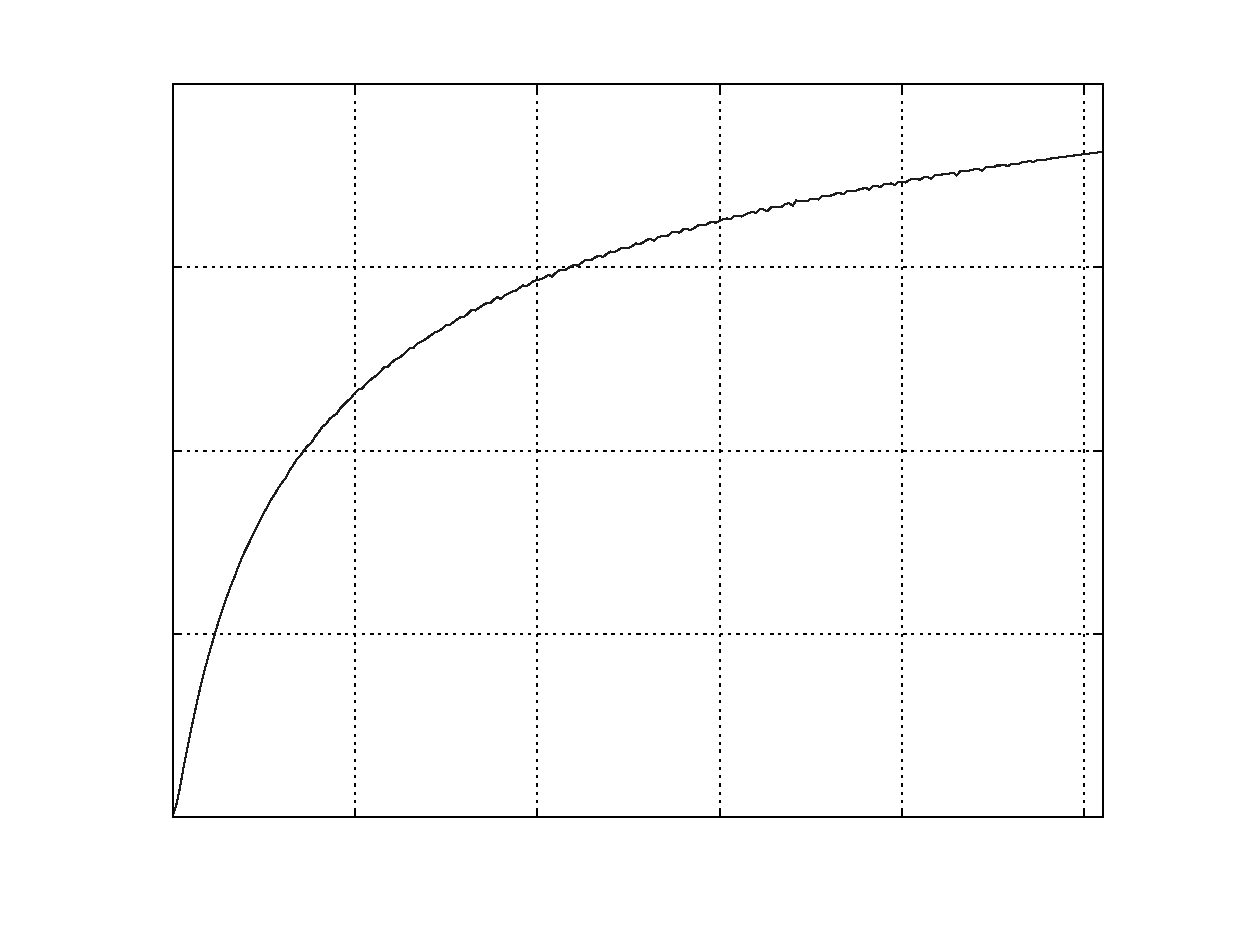
\includegraphics{img/steady_state-inc}
\end{picture}%
\begin{picture}(576,432)(0,0)
\fontsize{10}{0}
\selectfont\put(74.88,42.5189){\makebox(0,0)[t]{\textcolor[rgb]{0,0,0}{{0}}}}
\fontsize{10}{0}
\selectfont\put(162.409,42.5189){\makebox(0,0)[t]{\textcolor[rgb]{0,0,0}{{50}}}}
\fontsize{10}{0}
\selectfont\put(249.939,42.5189){\makebox(0,0)[t]{\textcolor[rgb]{0,0,0}{{100}}}}
\fontsize{10}{0}
\selectfont\put(337.468,42.5189){\makebox(0,0)[t]{\textcolor[rgb]{0,0,0}{{150}}}}
\fontsize{10}{0}
\selectfont\put(424.998,42.5189){\makebox(0,0)[t]{\textcolor[rgb]{0,0,0}{{200}}}}
\fontsize{10}{0}
\selectfont\put(512.527,42.5189){\makebox(0,0)[t]{\textcolor[rgb]{0,0,0}{{250}}}}
\fontsize{10}{0}
\selectfont\put(69.8755,47.52){\makebox(0,0)[r]{\textcolor[rgb]{0,0,0}{{0}}}}
\fontsize{10}{0}
\selectfont\put(69.8755,135.54){\makebox(0,0)[r]{\textcolor[rgb]{0,0,0}{{1}}}}
\fontsize{10}{0}
\selectfont\put(69.8755,223.56){\makebox(0,0)[r]{\textcolor[rgb]{0,0,0}{{2}}}}
\fontsize{10}{0}
\selectfont\put(69.8755,311.58){\makebox(0,0)[r]{\textcolor[rgb]{0,0,0}{{3}}}}
\fontsize{10}{0}
\selectfont\put(69.8755,399.6){\makebox(0,0)[r]{\textcolor[rgb]{0,0,0}{{4}}}}
\fontsize{10}{0}
\selectfont\put(298.08,31.5188){\makebox(0,0)[t]{\textcolor[rgb]{0,0,0}{{PWM value (0--255)}}}}
\fontsize{10}{0}
\selectfont\put(59.8755,223.56){\rotatebox{90}{\makebox(0,0)[b]{\textcolor[rgb]{0,0,0}{{Voltage at \texttt{A0} (\si{\volt})}}}}}
\end{picture}
}
    \caption{}
    \label{fig:}
\end{figure}

\begin{figure}[h]
    \centering
    \resizebox{\textwidth}{!}{% Title: glps_renderer figure
% Creator: GL2PS 1.3.8, (C) 1999-2012 C. Geuzaine
% For: Octave
% CreationDate: Tue Dec 29 00:54:08 2015
\setlength{\unitlength}{1pt}
\begin{picture}(0,0)
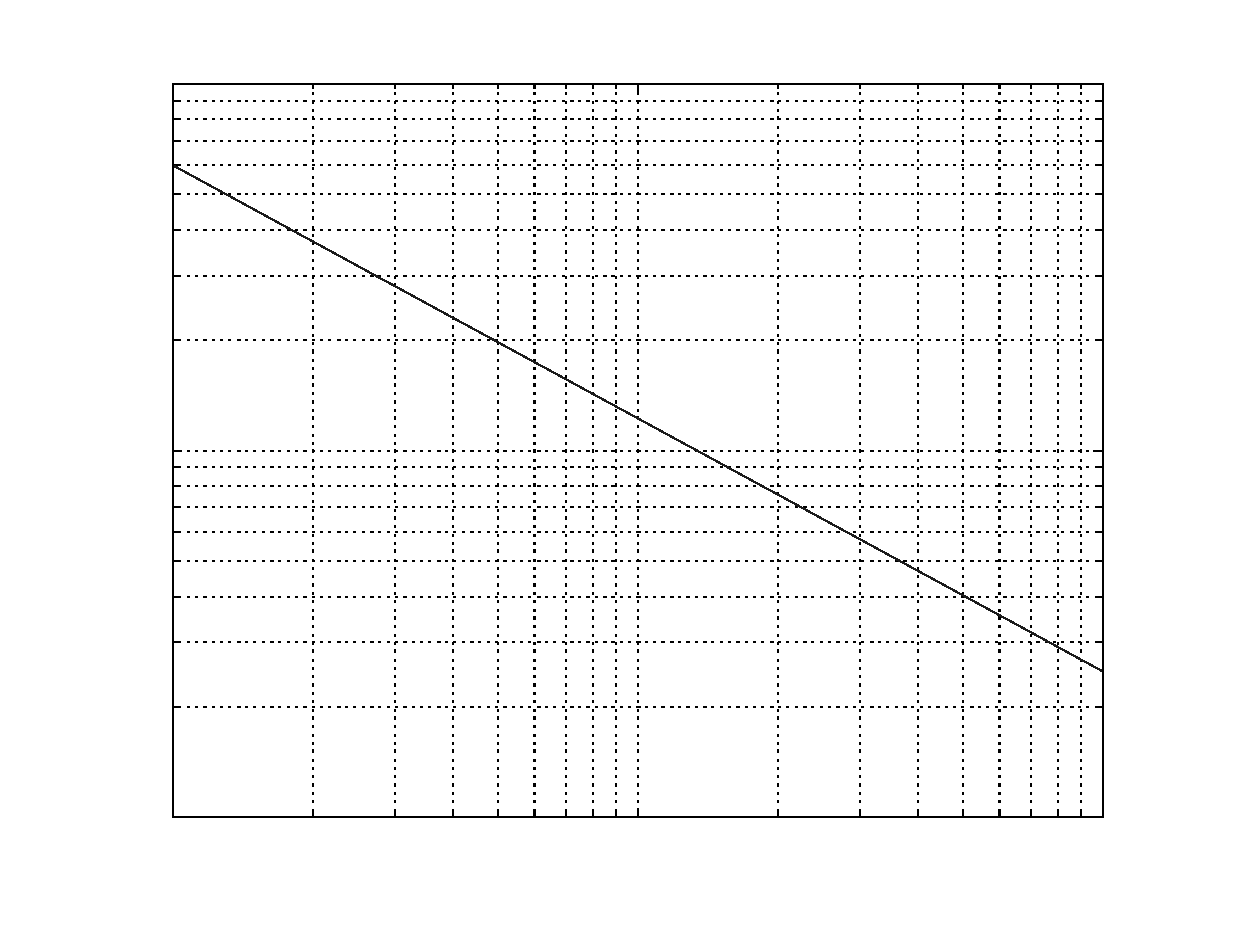
\includegraphics{img/LDR_model-inc}
\end{picture}%
\begin{picture}(576,432)(0,0)
\fontsize{10}{0}
\selectfont\put(74.88,42.5189){\makebox(0,0)[t]{\textcolor[rgb]{0,0,0}{{1e+0}}}}
\fontsize{10}{0}
\selectfont\put(298.08,42.5189){\makebox(0,0)[t]{\textcolor[rgb]{0,0,0}{{1e+1}}}}
\fontsize{10}{0}
\selectfont\put(521.28,42.5189){\makebox(0,0)[t]{\textcolor[rgb]{0,0,0}{{1e+2}}}}
\fontsize{10}{0}
\selectfont\put(69.8755,47.52){\makebox(0,0)[r]{\textcolor[rgb]{0,0,0}{{1e+3}}}}
\fontsize{10}{0}
\selectfont\put(69.8755,223.56){\makebox(0,0)[r]{\textcolor[rgb]{0,0,0}{{1e+4}}}}
\fontsize{10}{0}
\selectfont\put(69.8755,399.6){\makebox(0,0)[r]{\textcolor[rgb]{0,0,0}{{1e+5}}}}
\fontsize{10}{0}
\selectfont\put(298.08,31.5188){\makebox(0,0)[t]{\textcolor[rgb]{0,0,0}{{Illuminance (\si{\lux})}}}}
\fontsize{10}{0}
\selectfont\put(39.8755,223.56){\rotatebox{90}{\makebox(0,0)[b]{\textcolor[rgb]{0,0,0}{{Resistance (\si{\ohm})}}}}}
\end{picture}
}
    \caption{}
    \label{fig:}
\end{figure}

\subsubsection{Step Response}
\label{sub:StepResponse}

\subsubsection{Incremental Response}
\label{sub:IncrementalResponse}

\subsubsection{LDR to Lux}
\label{sub:LDRtoLux}

\begin{figure}[h]
    \centering
    \resizebox{\textwidth}{!}{% Title: glps_renderer figure
% Creator: GL2PS 1.3.8, (C) 1999-2012 C. Geuzaine
% For: Octave
% CreationDate: Tue Dec 29 00:58:25 2015
\setlength{\unitlength}{1pt}
\begin{picture}(0,0)
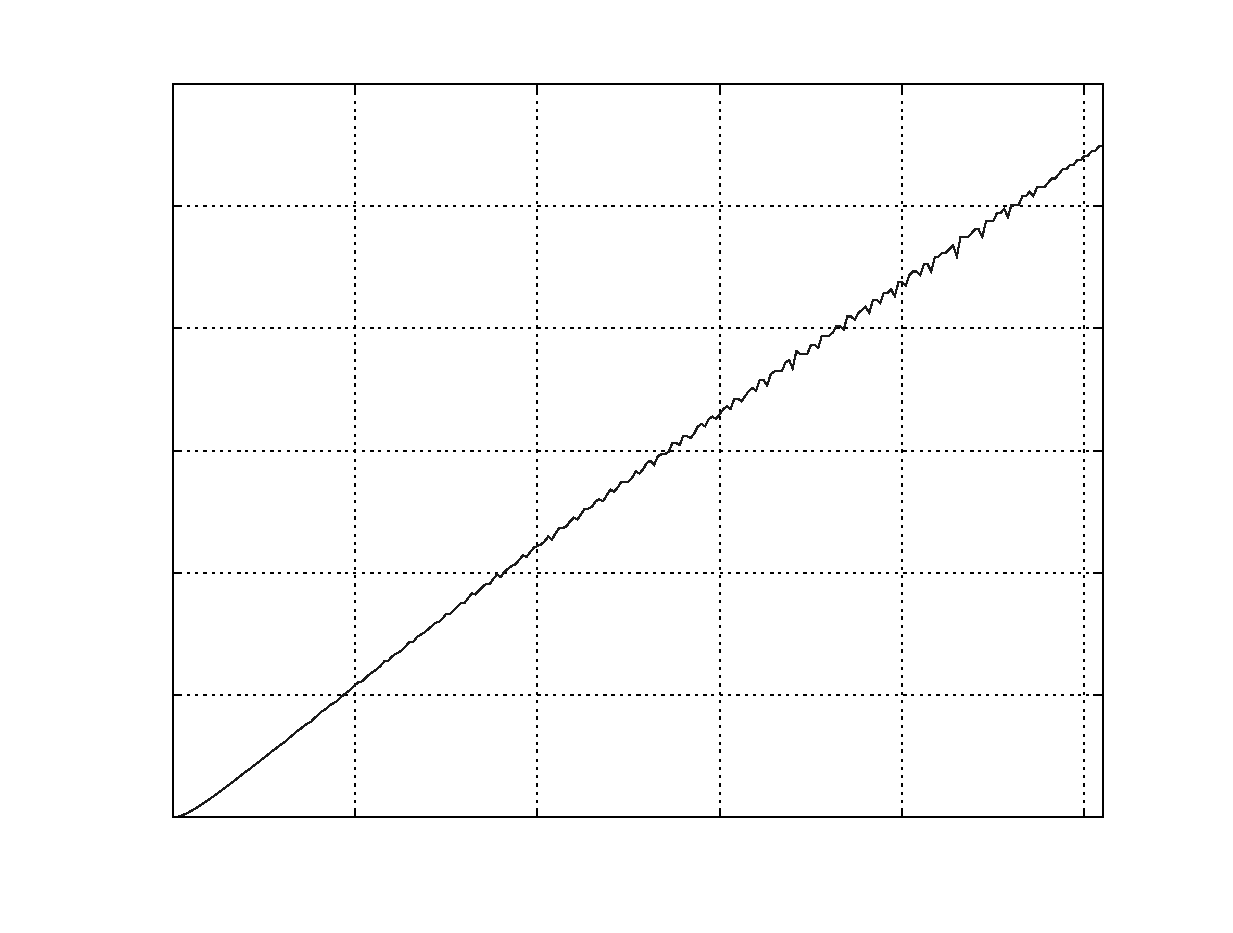
\includegraphics{img/pwm_to_lux-inc}
\end{picture}%
\begin{picture}(576,432)(0,0)
\fontsize{10}{0}
\selectfont\put(74.88,42.5189){\makebox(0,0)[t]{\textcolor[rgb]{0,0,0}{{0}}}}
\fontsize{10}{0}
\selectfont\put(162.409,42.5189){\makebox(0,0)[t]{\textcolor[rgb]{0,0,0}{{50}}}}
\fontsize{10}{0}
\selectfont\put(249.939,42.5189){\makebox(0,0)[t]{\textcolor[rgb]{0,0,0}{{100}}}}
\fontsize{10}{0}
\selectfont\put(337.468,42.5189){\makebox(0,0)[t]{\textcolor[rgb]{0,0,0}{{150}}}}
\fontsize{10}{0}
\selectfont\put(424.998,42.5189){\makebox(0,0)[t]{\textcolor[rgb]{0,0,0}{{200}}}}
\fontsize{10}{0}
\selectfont\put(512.527,42.5189){\makebox(0,0)[t]{\textcolor[rgb]{0,0,0}{{250}}}}
\fontsize{10}{0}
\selectfont\put(69.8755,47.52){\makebox(0,0)[r]{\textcolor[rgb]{0,0,0}{{0}}}}
\fontsize{10}{0}
\selectfont\put(69.8755,106.2){\makebox(0,0)[r]{\textcolor[rgb]{0,0,0}{{10}}}}
\fontsize{10}{0}
\selectfont\put(69.8755,164.88){\makebox(0,0)[r]{\textcolor[rgb]{0,0,0}{{20}}}}
\fontsize{10}{0}
\selectfont\put(69.8755,223.56){\makebox(0,0)[r]{\textcolor[rgb]{0,0,0}{{30}}}}
\fontsize{10}{0}
\selectfont\put(69.8755,282.24){\makebox(0,0)[r]{\textcolor[rgb]{0,0,0}{{40}}}}
\fontsize{10}{0}
\selectfont\put(69.8755,340.92){\makebox(0,0)[r]{\textcolor[rgb]{0,0,0}{{50}}}}
\fontsize{10}{0}
\selectfont\put(69.8755,399.6){\makebox(0,0)[r]{\textcolor[rgb]{0,0,0}{{60}}}}
\fontsize{10}{0}
\selectfont\put(298.08,31.5188){\makebox(0,0)[t]{\textcolor[rgb]{0,0,0}{{PWM value (0--255)}}}}
\fontsize{10}{0}
\selectfont\put(53.8755,223.56){\rotatebox{90}{\makebox(0,0)[b]{\textcolor[rgb]{0,0,0}{{Measured illuminance (\si{\lux})}}}}}
\end{picture}
}
    \caption{}
    \label{fig:}
\end{figure}


% From first report:

%Os seguintes pontos descrevem o que é implementado no código actual:
%Controlador com componentes proporcional, derivativa e integral
%Anti-windup
%Feedforward
%Derivador à saída
%Temporização do controlador através de interrupções
%Dar referências em lux
%Medir iluminância em lux
%Alterar parâmetros do controlador
%Alterar tempo de amostragem
%Implementamos um filtro passa-baixo para o derivador para diminuir o ruído. Não chegámos a afinar a constante desse filtro, pelo que o temos comentado.
%Os parâmetros do controlador foram encontrados com afinação manual e são os seguintes:
%Ganho proporcional: 10
%Ganho diferencial: 0.01
%Ganho integral: 10
%Ganho do feedforward: 0.1
%Ganho do anti-windup: 0.05
%Tempo de amostragem: 1500 µs
%Todos os cálculos do controlador são feitos com valores de 0 a 1023, sendo convertidos quando necessário: para 0 a 255 para actuar o LED; e para lux quando são pedidos valores de iluminância.

\subsection{Local Controller}
\label{sec:LocalController}

The local controller consists of a Proportional-Integral-Derivative Controller (PID) that receives as input a integer reference value (\emph{r}) from 0 to 1023, the LDR readings from 0 to 1023 (\emph{y}) and has as output the PWM duty cycle (\emph{u}) in the range 0 to 255.

The block diagram of the local controller is on Figure~\ref{fig:pid_block_diagramm}. The error(\emph{e}) is defined as $e = r - y$. The signal \emph{u} is calculated as the sum of the proportional, integral and derivative components and the feedforward term.

\begin{figure}[!h]
	\centering
		\includegraphics[scale=0.8]{img/pid_block_diagramm}
	\caption{Locall controller block diagram}\label{fig:pid_block_diagramm}
\end{figure}


\subsubsection{Proportional Component}
\label{sub:ProportionalComponent}

The proportional component of the controller is just a gain multiplied (\emph{$K_p$}) by \emph{e}. $ P = K_p * e$.

\subsubsection{Integral Component}
\label{sub:IntegralComponent}

\subsubsection{Derivative Component}
\label{sub:Derivative Component}

The derivative component is calculated as $ D = - K_d/T_s * (y_{t}-y_{t-1})$. This component is calculated with signal \emph{y} instead of \emph{u} to avoid differentiating discontinuities, which would cause the signal \emph{u} to saturate.

\subsubsection{Anti-Windup}
\label{sub:AntiWindup}

\subsubsection{Feedforward}
\label{sub:Feedforward}

\subsubsection{Implementation Details}
\label{sub:Implementation Details}

This controller was implemented as a interrupt routine to guarantee its execution in fixed intervals.

\subsubsection{Parameters}
\label{sub:Parameters}

\subsection{Server}
\label{sec:Server}

\subsection{Simplex}
\label{sec:Simplex}

The Simplex algorithms solves Linear programms, it finds the optimal solution if it exists.
We implemented the simplex following the pseudo-code on the book \emph{Introduction to Algorithms} \cite{Cormen}.
This implementation solves Linear programms of the form:

$$ \text{max }c*x $$
$$    A*x \geq b, $$
$$    x \geq 0 $$

We can describe the problem as a Linear programm of this form. First we define \emph{O} as the array with the external illuminance at each \emph{desk}, \emph{l} as the array with the desired illuminance for each \emph{desk} and \emph{E} as the  3 by 3 matrix of influence between each light. The problem we want to solve is to find the minimal values for \emph{d}, the PWM values normalized from 0 to 1, that make the illuminance be equal to \emph{l}.


Note: To throughly test the Simplex implementation a series of simple unit tests were constructed using the \emph{Boost Test} Library.

\subsection{Serial Communications}
\label{sec:SerialCommunications}


\section{Experiments}

To analyze the resulting system 3 metrics were implemented (as specified on the assignment):
\begin{itemize}
    \item Energy: the energy consumed at each desk assuming each LED has a nominal power of 1W
%$$ E = \sum_{i=2}^{N} d_{i-1}(t_{i-1}-t_i) $$

    \item Comfort error: the average error between the reference illuminance and the measured
illuminance for the periods when the measured illuminance is below the reference

    \item Comfort variance: the average variation of the illuminance during periods of constant occupation computed by and approximation to the second derivative of the illuminance.
\end{itemize}

We used these metrics to evaluate the system's performance on our experiments. First to test the Local Controller operation with multiple Arduinos working simultaneously we ran two experiments. The results of these experiments are presented and discussed on \autoref{results}.

With the box closed (no external lighting) and with all desks set as unoccupied (reference of \SI{15}{\lux}) we analyzed the three metrics on the first 6 seconds after system startup.

With the box slightly open (some external lighting) and with the first and the third desks set as occupied (reference of \SI{30}{\lux}) we analyzed the metrics in the same way.

The values for the occupied and unoccupied reference were chosen taking into consideration \autoref{fig:pwm_to_lux}.

\section{Results \& Discussion}

Great Results:

\section{Conclusion}
\label{conclusion}

The final results of this project constitute a control system that allows to control ambient light to meet desired levels specified according to the occupation of parts of a room. The system includes a server that can be connected to a network of luminaires allowing to control the references of each as well as acquired data to measure the energetic efficiency and comfort metrics of the illumination system.

One contribution of this work is the implementation of an interrupt based PID controller that runs on a common microcontroller. Another important contribution is the implementation of the Simplex algorithm according to the pseudocode presented in \cite{Cormen}. This implementation includes the needed transformations for cases where the initial solution is unfeasible. No previous implementation that follows this work was found to exist.

The use of the results provided by the simplex failed to improve the system. Even when the results of the simplex algorithm are applied the system evolves naturally to the state it was before. That state satisfies the illumination requirements but is proved not to be optimal energy-wise.

There is room to improve several aspects of the system. Namely the protocols used could be more robust; the ATmega ADC noise reduction mode could be used to acquire better samples; and the ADC readings could be made in the background by using the interrupts that exist for that purpose and a circular buffer instead of using \texttt{analogRead()} several times and make a mean of the values to filter some noise.



 %
 %Conclusions summarize	the main    achievements    
 %of  the	work.
 %• Also	identify    other   aspects that    are	relevant    for	
 %other	researchers.
 %• Stress    the	contributions	and how	the world   will    
 %be  a	much	better	place	to  live    after   your    work.
 %• Mention   a	few points  worth   looking at	in  future  
 %work,	as  a	consequence of	the conclusions.



\pagebreak
% references
\nocite{*}
\bibliography{references}
\bibliographystyle{abbrv}

\end{document}
